\chapter{Background}
\label{sec:metrics}

This chapter describes background knowledge required to understand the remaining parts of the thesis. It introduces the target system for this work as well as datasets and metrics used for evaluation. Furthermore, it discusses related work in Object Detection and Data Generation.


\section{Detecting Objects}
\label{sec:object_detection:related}

On a high level Object Detection can be described by two individual goals: the description of what kind of object is seen (Classification), as well as where it is seen (Localization). Hence, an Object Detection pipeline transforms the raw image to a set of one or more areas and corresponding class labels. Images are high dimensional signals that can contain redundant and task irrelevant information. Performing detection in this space is difficult, also because the performance of machine learning models decreases when the feature space becomes too large (curse of dimensionality), Computer Vision pipelines usually apply a feature extraction stage, before the actual prediction is done. An overview is displayed in \Cref{fig:obj_pipeline}.

\begin{figure}[hbtp]
	
	\centering
	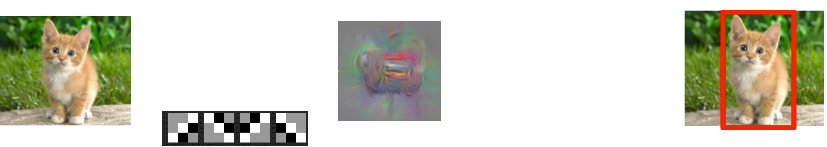
\includegraphics[width=\linewidth]{fig/ObjectDetection}
	\caption{Object Detection Pipeline. An initial step extracts task relevant features of the input signal and derives an internal representation. Consecutively, classification determines what kind of object is present in the image, while localization determines where the object is located. The output consists of area(s) with class annotation.}
	\label{fig:obj_pipeline}
\end{figure}
\begin{enumerate}
	\item The feature extraction stage extracts task relevant information from the image and infers an internal, more abstract representation of lower dimension.
	
	\item The classification/localization stage produces the final output based on this representation. 
	\todo{add object model}
\end{enumerate}

An efficient feature extraction stage is thereby crucial for the success of an Object Detection pipeline. If the inferred representation is clearly separable, a simple classification stage can distinguish an object from the background. In contrast, even a flexible classifier cannot separate a highly overlapping feature space.

\subsection{Baseline Algorithm}

The above pipeline can be illustrated in the example of the baseline algorithm of this work: \textit{SnakeGate}. Its scheme is summarized in \todo{text} and described here on a higher level.

Initially, the image gets filtered by a higher and lower color threshold. This way ideally the largest part of pixels in the image is removed. This can be seen as the feature extraction stage.

In the resulting binary image the follow up stage searches for object parts. \textit{SnakeGate} detects square objects and hence looks for vertical and horizontal bars that are respectively perpendicular to each other. Once this combination is found in a particular area of the image, it is counted as a valid detection. In the final step the corners of the bounding box are refined to get more accurate coordinates.

This simple method shows how crucial the feature extraction stage is. With a suitable color threshold, object parts can easily be found and the detection is accurate. However, this requires an evenly distributed colour across the object. As soon as back light or shadows fall on the object, a clear separation is difficult. Therefore, \textit{SnakeGate} is quite subtle to light changes.

Another issue of \textit{SnakeGate} is that it is defined as 4 bars in quadrangle shape. If one of the bars is not clearly visible the algorithm can not detect detect the object. Also, it does not exploit object context such as the object pole.

\begin{enumerate}
	\item Filter image by colour threshold
	\item Sample stochastically 
	\item Follow the pixels horizontally as long as they are within the colour threshold otherwise return to 2.
	\item If a bar of sufficient length has been found repeat 3. vertically along one end of the line found in 3.
	\item If a vertical bar is found the square is considered as gate candidate
	\item Create local histogram around the corners of the gate candidate and choose the highest peak as gate corner.
	\item Count the fraction of pixels within the color threshold  in relation to the total number of pixels a long all edges of the gate candidate to determine the \textit{color fitness}.
	\item Gate candidates that exceed a chosen threshold are considered valid detections.
\end{enumerate}
\todo{this can be described more formally}


\subsection{Related Work}

The problems of \textit{SnakeGate} are very typical for Object Detection. Since the beginning researchers investigated different methods of feature selection and the definition of object models. While initial work manually defined such features, later work replaced many of these stages with learning based methods. Today, whole state-of-the-art pipelines can be trained directly on raw images. This section investigates available literature and discusses the major milestones relevant for this work.

\subsubsection{Traditional Methods}

The early attempts to Object Detection define objects in terms of basic volumetric shapes such as cubes and cylinders. During inference these features are extracted and compared to a database. However, in practice even recognizing these basic shapes proves to be difficult \cite{Andreopoulos2013}. 

Later approaches focus more on appearance based features such as wavelets \cite{Papageorgiou} which also applied in \cite{Viola2004} for human face detection. Thereby the image is processed by a cascade of classifiers using a sliding window in multiple scales. The processing of an image patch is stopped when a patch is classified as background. The features can be computed with simple operations and thus the detector can be executed extremely fast. Yet, the used Haar-wavelets cannot efficiently encode complex textures making the approach less suitable for many real world objects \cite{Andreopoulos2013}. 

In contrast, \ac{HOG} \cite{Dalal} and \ac{SIFT} \cite{Lowe2004} use the image gradient to cover shape information. In a sliding window local histograms based on the gradient orientation are calculated. \citeauthor{Dalal} \cite{Dalal} use the feature for pedestrian detection.

A general challenge in Computer Vision is the combination of local image features such as corners and edges to a more global detection of an object. Especially, when parts of the object can be occluded or deformed and thus undergo variations in appearance. In order to cope with these issues \citeauthor{Felzenszwalb} \cite{Felzenszwalb} model pedestrians in individual parts and combine them in their proposed \ac{DPM}.

Traditional methods have in common that the individual steps of the detection pipeline are optimized separately. Furthermore, often the feature extractors and object models are designed manually. Hence, designing such a detector can result in cumbersome application dependent work. \ac{EWFO} have sparse features and cameras on \ac{MAV} can have a strong influence on the object appearance. Modelling this appearances manually is difficult. Also, the methods seem to have reached a limit in performance in the years of 2005-2012 where almost no improvement in performance was achieved.

\subsubsection{\acp{CNN}-based Feature Extraction}

A breakthrough in detection performance came with \acp{CNN} which emerged from Deep Learning research and subsequently became a popular feature extractor. \acp{CNN} can be seen as small neural networks that are applied locally on image patches in sliding window fashion. The outputs of the initial local operations (first layer) are further processed by higher layers until the desired output size is reached. The model parameters (weights) are trained using a loss function and the back-propagation algorithm.

The modular structure of \acp{CNN} allows to create highly non-linear models that can represent any function. However, this flexibility also introduces the challenge of choosing a suitable architecture. On a fundamental level design parameters can be summarized in depth, width and kernel size. 

\Cref{fig:model_design} displays these parameters and introduces additional terminology necessary for the remaining parts of this chapter. The \textit{kernel size} $\textbf{k}$ determines the spatial size of a kernel and therefore how big the patch is, the convolution is applied on. A layer usually contains multiple filters that are applied on its input. The amount of filters is also referred to as \textit{width} $w$. The filters are applied in sliding window fashion which introduces the step size ( \textit{strides} $\mathbf{s}$) as an additional parameter. The output of each convolution is concatenated and processed by the next layer. The amount of layers is also referred to as \textit{depth}. In the image also the \textit{receptive field} of a filter is visualized. This describes the image patch that is related to a certain feature response. The filter of the first layer (green) has a receptive field corresponding to its kernel size. The filter of the second layer (blue) combines the responses of the filters of the first layer at multiple spatial locations an thus has an increased receptive field.

\begin{figure}[hbtp]
	\centering
	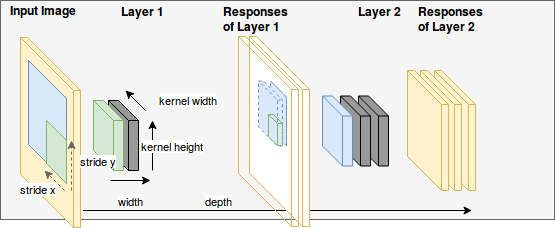
\includegraphics[width=0.8\textwidth]{fig/model_design}
	\label{fig:model_design}
	\caption{Notation in \acp{CNN}. The input image is convolved with a layer. One layer contains multiple kernels that are convolved in sliding window fashion with certain step size. The responses of the convolutions are collected and processed by the next layer. The receptive field is determined by which parts of the input image are part of the kernel response at layer x. The total amount of layers is also referred to as depth.}
\end{figure}

Among these parameters depth is considered one of the preliminary parameters to improve performance \cite{He}. \citeauthor{Simonyan2014} \cite{Simonyan2014} achieve first places in the 2014 ImageNet Classification challenge using a network that only contained filters of size 3-by-3 but up to 19 layers. \citeauthor{Szegedy2014} \cite{Szegedy2014} achieve similar performance using a network with 22 layers. The proposed network included an \textit{Inception}-module, an architectural element that allows deeper networks at a constant computational budget. 


\paragraph{Fully Convolution Networks.}

Instead the work focuses on much smaller networks that are fast to execute. Execution time is also the motivation for \acp{FCN}. Instead of using a fully connected layer in the last stage, these networks only apply local operations. This saves many computations in the last layer and enables the application of models on various input sizes.

\paragraph{Dilated Convolutions.}

However, \ac{FCN} in combination with a small amount of layers introduce a limited receptive field. If the network is too shallow the last layer cannot take into account the whole input image. A way to increase the receptive field without increasing the number of computations is the use of sparse kernels, also called Atrous/Dilated convolutions. 

\paragraph{Depthwise Separable Convolutions.}

Another line of research to reduce the number of computations in \acp{CNN} address the convolution operation. \textit{MobileNet} \cite{Howard2017} and \textit{QuickNet} \cite{Ghosh2017} make extensive use of \acp{DSC}. \acp{DSC} replace the original 3D-convolution by several 2D-convolutions followed by a pointwise convolution. This reduces the total number of operations from $N = k_w \cdot k_h \cdot w_n \cdot w_{n+1}$ to $N=(k_w \cdot k_h + w_n)+w_n \cdot w_{n+1}$. \textit{MobileNetV2} \cite{Sandler2018} further includes linear bottlenecks to reduce the total number of operations. These are convolutions with a 1by1 kernel and linear activation.

\paragraph{Channel Shuffling.}

\cite{Zhang2017a} addresses the computational costs of pointwise convolutions. Instead of applying a pointwise convolution on the whole input volume, group convolutions are applied on by dividing the channels in subsets. These channels are shuffled to enable cross-channel information propagation. 

Despite a large amount of research conducted in finding suitable architectures there has not yet been a single way that always achieves a goal. It has been shown how models with a large amount of parameters combined with vast amounts of training data perform well on various vision tasks and objects. However, there is no guarantee that the found representation is also the most suitable/efficient one. The research resulted in a collection of rules an best practices that need to be considered with the task at hand. This work investigates the design of a \ac{CNN} for the detection of \ac{EWFO}.

\subsubsection{\ac{CNN}-based Object Detection}

After showing promising results for Classification, \acp{CNN} where also applied for Object Detection. \acp{CNN}-based Object Detectors can broadly be grouped in two categories. The categories are introduced and finally compared in relevance to this work.

\paragraph{Two-Stage Detectors.}

\citeauthor{Girshick2013} \cite{Girshick2013} use Selective Search \cite{Uijlings2013} to extract object candidates from an image and classify each region with a \ac{CNN}. However, this requires to run the whole network at various scales and overlapping locations. Hence, the approach is computationally intense while many of the performed operations are redundant.

Follow up work aims to share computations for faster inference. Spatial Pyramid Pooling \cite{He2014b} allows to crop any region to a predefined size. Thus a \ac{CNN} does not have to be run at overlapping regions anymore but the extracted features can be reused and need to be only computed once. This leads to a vast reduction in computations and leaves the region proposal algorithm as a computational bottleneck.

With the \ac{RPN}\cite{Ren2015} region proposals and feature extraction is combined in a single stage. The whole stage is framed as a regression problem by predicting object probability for a predefined set of bounding boxes so called anchor/prior or default boxes.  Predefining the total amount of possible locations and bounding box dimensions would lead to an intractable amount of parameters and computations. Hence, the most common object appearances are defined and the network not only predicts an object probability for each box but also how to adapt location and dimensions to better fit the predicted object. Combining feature extraction and region proposals in a single network led to 213x speed up at that time.
 
Being currently the method with the best performance in terms of \ac{mAP} two stage approaches would be a valid choice for the detection of \ac{EWFO}. However, their two stage character makes the inference time relatively slow, which is not suitable for the application on a \ac{MAV}. Also, this work investigates the detection of a single object. For this application the \ac{RPN} can be used directly.

\paragraph{One-Stage Detectors.}

One stage detectors aim to further combine multiple stages of the Object Detection task into a single network. Therefore the whole pipeline is framed as a regression task. This leads to the question how to discretize the input image. 

The first one stage detector \ac{Yolo}\cite{Redmon} divides the input image in a fixed grid and predicts class probabilities for each grid cell. As this limits the amount of bounding box coordinates significantly the network also predicts global bounding box coordinates and a object probability for each box. As a last step a postprocessing algorithm fuses the output to the final prediction. Being a breakthrough as the first one stage detector the approach is limited to predict a single class for each grid cell. Furthermore, the approach of predicting bounding box coordinates globally proved hard for the network to learn and resulted in high localization errors.

Better results could be achieved by predicting offsets to predefined regions as in the concept of the aforementioned anchor boxes. \ac{SSD} \cite{Liu} extends the anchor box approach to perform the whole Object Detection task. Therefore the network not only predicts bounding box coordinate offsets and object probability but also a class probability for each anchor box. 

An issue that arises with discretization of the object detection task is that objects can appear at different scales. For small objects it is required to have a high resolution of bounding box locations to have a sufficient representation of the input image. For example many small objects can appear next to each other. A too coarse resolution could not capture the fact that there are multiple objects present. Furthermore, it is required to take into account fine grain features to predict such an object. In contrast, for large objects small changes in location do not make a difference. In contrary, a too fine resolution can cause the detector focus on noise and thus lead to bad predictions or unstable training. Therefore, \ac{SSD} introduces the prediction of objects at multiple output grids at different layers of the network. Thus, the output grid can be defined depending on the object size and the network can extract features based on the object scale. Follow up work in \cite{Redmon, Redmona} also included the concept of anchor boxes and prediction layers at multiple scales, making \ac{SSD} and \ac{Yolo} converge to a very similar solution.


In \cite{Huang} one and two stage detectors are compared in terms of accuracy as well as resource requirements. While two stage detectors with very deep networks tend to achieve the best performance, one stage detectors are generally faster. The experiments also show how the inference time of two stage detectors can be reduced without loosing too much accuracy when the amount of bounding box proposals is limited. However, single shot detectors are still the fastest method with the lowest memory profile. Furthermore, for the single class case the region proposal stage of a two stage detector can be used directly. Hence, in this work we investigate the detection of a \ac{EWFO} with a one stage detector. 

The anchor box concept allows to incorporate prior knowledge about possible objects but also introduces additional hyperparameters that need to be tuned for an application. Therefore the alternative approach of \textit{CornerNet}\cite{Law2018} avoids the anchor box concept by defining objects as paired key points. Each bounding box is defined as two corners. The network predicts a heatmap with potential corner locations as well as which corners belong together. This would be an interesting approach for the detection of \ac{EWFO}. However, as the publication was quite recent the approach could not be taken into account. 

\subsubsection{Attention Models}

A research direction which is fundamentally different to the approaches seen so far are models based on visual attention. Instead of processing the whole input image at once, the aim is to process only relevant image patches. Typically a model processes an image crop and decides which location to evaluate next until enough information is gathered for the final prediction. Examples for the approach can be found in \cite{Itti1998,Ba2014,Ablavatski2017a}.

Attention models are promising as their computational complexity can be controlled independently from the number of pixels in the input image. However, to this end successes have mostly been demonstrated on digit recognition like the MNIST dataset. Scaling the approach to real world problems proves to be difficult. Furthermore, the features of an \acp{EWFO} are sparse, while most part of the image does not provide hints where to look for an object. Therefore, we assume the approach less applicable for the detection of \acp{EWFO}.

\subsection{Reducing Inference Time}

Computer Vision research typically focuses on detection accuracy rather than inference speed. However, for the deployment on a \ac{MAV} resource consumption is an important parameter. The following describes research topics that concern the reduction of inference time.

\todo{cleanup}
One pass of the state of the art \ac{CNN} ResNet101 contains of 11.3 billion floating point operations. Even assuming a powerful 2 GHz processor can perform 2 billion calculations per second it would still require almost 6 seconds for one network pass. Furthermore, a \acp{CPU} usually has to reload operands from the memory and cannot directly perform floating point multiplications. Hence, the actual forward pass would require even more time.


Therefore researchers address the reduction of inference time by reducing the number of operations. For example MobileNet and ShuffleNet aim to reduce the computations by addressing the expensive 3D convolutions. Other researchers aim to making the individual operations more efficient. This can be done by replacing floating point operations with integer operations hence quantizing the network.

In order to infer a layer in a \acp{CNN} kernels are convolved at multiple locations within one image. Thereby the same calculations are applied on various input data while the individual operations are independent of each other. Hence, theoretically the computations in one layer can be performed completely in parallel. The output of one layer can be stored similarly to the input image as a matrix. Computational platforms that exploit this fact are \acp{GPU} that have been adopted for Deep Learning applications from early on. In contrast to \acp{CPU} that are optimized to perform many different operations sequentially, \acp{GPU} typically consist of more cores and are optimized to perform the same operation on different data. While each individual core is typically slower than a single core in a \acp{CPU}, \acp{GPU} are much faster for applications that can be performed in parallel.

With a large enough \ac{GPU} it does not matter whether an operation is performed at an image of size 150x150 or 300x300 despite the actual computations increase by a factor of 4. However, such powerful \acp{GPU} require space and energy which is typically not available for small scale \acp{MAV}. The JeVois Smart Camera contains a MALI-400GPU with two cores and 408 Mhz each. Additionally it contains floating point registers and supports NEON operations. These are processor instructions that enable the efficient use of \acp{SIMD} operations.

The actual inference time of a network strongly depends on the computational platform, memory access times as well as the particular low level implementation. Hence, the number of computations within a network can only give a limited insight on the actual inference time. For example the \textit{TensorflowLite} framework allows the deployment of models created in \textit{tensorflow} on mobile processors. However, with this framework a the application of a single kernel on a 104x104 input volume takes 27.1 ms on the JeVois. In contrast, the same operation performed with the \textit{Darknet} framework that supports NEON operations takes only 5.07 ms. 


\subsubsection{Weight Quantization}

The hardware of most embedded \ac{CPU} support only integer operations and thus rely on software to perform floating point operations. Hence, weight quantization is another line of research to reduce the inference time of deep networks on mobile devices. By mimicking the quantization effects during training, the network learns to deal with these kind of artefacts. However, the target platform of this work supports hardware accelerated floating point multiplications. While weight quantization could still be used to accelerate the network it would require serious low level operation optimization. This work addresses the optimization on a more high level architectural basis.
\todoref{put some refs where this is applied \cite{TripathiSanDiego}}

\subsubsection{Knowledge Distillation}

Knowledge Distillation \cite{Hinton2006} is way to create a smaller model based on a trained bigger model or an ensemble of models. Thereby the smaller student-network is trained to mimic the output of the final and intermediate activations of the teacher-network. \textit{FitNet} extends the approach to create a thinner/deeper network based on a trained network thereby reducing parameters without loosing performance. In \cite{Li2017c} the approach is applied to the task of Object Detection. In \cite{Wei2018a} knowledge distillation is combined with weight quantization in order to obtain a faster and more efficient model.

The approaches have in common that a very complex function learned from a deep model is aimed to be compressed in a more efficient model. Training the smaller model directly leads to a lower performance than using the distillation approach. We assume this is successfully as the network architectures used are generally deep. Even \cite{Wei2018a} which speaks of very tiny networks uses the VGG-architecture with 23 layers. These architectures are prohibitive to be deployed on small scale \acp{MAV}. We investigate a network size of around 10 layers. Such networks are easier to train and our experiments how we can reduce the width of the model by simply training the network on the task. Therefore we do not investigate this approach further.

\section{Generating Data}
\label{sec:training:related}

Related methods vary from changing low level properties of the image over using CAD models in combination with real background up to rendering full 3D-environments. Often various combinations of synthesized and real data are applied. 

\subsubsection{Low-Level Image Augmentation}

A common part of current Computer Vision pipelines is to augment a given data set by transforming low level properties of the image. By artificially increasing variations in the input signal, a model that is more invariant to the augmented properties shall be obtained.

\citeauthor{Krizhevsky2012a} \cite{Krizhevsky2012a} use \ac{PCA} to incorporate colour variations. \citeauthor{Howard2013} \cite{Howard2013} shows how several image transformations can improve the performance of a \ac{CNN}-based Classification model. The proposed pipeline includes variations in the crop of the input image as well as variations in brightness, color and contrast. In \ac{CNN}-based Object Detection \citeauthor{Redmon} \cite{Redmon} uses random scaling and translation of the input image, as well as random variations in saturation and exposure. \citeauthor{Liu} \cite{Liu} additionally crop and flip each image with a certain probability.

Since most methods use image augmentation and \citeauthor{Krizhevsky2012a} \cite{Krizhevsky2012a} mentions it to be the particularly reason for superior performance at ILSVRC2012 competition it can be assumed to be beneficial for Computer Vision models. Unfortunately, none of the publications measures the improvements gained by the different operations. 

While the aforementioned approaches add artificial variation to the input data, \citeauthor{Carlson2018}\cite{Carlson2018} augment the image based on a physical camera model. The proposed pipeline is applied for Object Detection and incorporates models for sensor and lens effects like chromatic aberration, blur, exposure and noise. While being of minor effect for the augmentation of real data (0.1\% - 1.62\% \ac{mAP}70) the reported results show an improvement when training on fully synthesized datasets. Here the reported gains vary between 1.26 and 6.5 \% \ac{mAP}70.

Low-level image augmentation is a comparatively cheap method to increase the variance in a dataset. However, it cannot create totally new samples or view points. Furthermore, it cannot change the scene in which an object is placed. Therefore it needs a sufficiently large base dataset that is augmented. This work addresses the case when no real training data is available. Hence, low-level image augmentation is incorporated in the training process but can not be the only method applied.

\subsubsection{Augmenting Existing Images with CAD - Models}

In order to create new view points \ac{CAD}-models can be used. These models describe 3D-shape of an object and can be placed on existing images to augment or increase a dataset.

\citeauthor{Peng}\cite{Peng} study the use of \ac{CAD}-models in the context of \ac{CNN}-based Object Detection. The authors particularly address how image cues like texture, colour and background affects the detection performance. The experiments show how the used \acp{CNN} are relatively insensitive towards context but use shape as primary, texture and colour as secondary most important features. This enables competitive performance even when the object of interest is placed only on uniformly covered backgrounds. However, the study only covers solid objects such as birds, bicycles and airplanes. \ac{EWFO} are substantially different and we hypothesize that other image cues must be relevant.

\citeauthor{Madaan2017}\cite{Madaan2017} study the segmentation of wires based on synthetic training. As wires similarly to \ac{EWFO} only consist of thin edges, the application is quite close to this work. However, the experiments focus on a single domain, namely sky images and thus the variations in background are comparatively small. We hypothesize that \ac{EWFO} are particularly sensitive to such variations and address the application in multiple domains.

\citeauthor{Hinterstoisser2017} \cite{Hinterstoisser2017} propose to use a base network that has been trained on real images and to continue training on images with \ac{CAD}-models. During training the base network is frozen and only the last layers are updated. The method does not use real data but requires a suitable base network. As most available feature extractors (further discussed in \Cref{sec:object_detection}) are of a size that is computationally prohibitive for \ac{MAV} the method is not really applicable for this work. 

The use of CAD-models in combination with real backgrounds allows to generate totally new view points for the object of interest. Furthermore, the image background consists of real data and thus the synthetic textures only concern the rendered object. However, the geometric properties like perspective as well as the physical properties like object placement are violated and therefore create an artificial scene. Despite this fact, literature shows that such images can benefit model performance in various cases. Yet, most of the approaches still use real data and/or focus on solid objects with rich textures and complex shape. We hypothesize that since \ac{EWFO} do not provide these kind of structures the results do not apply in the same way. Hence, we incorporate the method to generate data and investigate how it can be applied for the detection of \ac{EWFO}.

\subsubsection{Fully Synthesizing Environments}

A more realistic placement of objects can be achieved when fully synthesizing environments.  The object of interest can be placed according to physical laws, shadows fall correctly and geometric properties of an image are followed. However, if the graphical models do not fully capture the details of real world objects, the generated data might look too artificial.

\citeauthor{Johnson-Roberson2016} \cite{Johnson-Roberson2016} use a powerful graphical engine and a highly detailed environment to train an Object Detection model entirely in simulation. The results show an improvement towards data annotated by humans especially when using vast amounts of simulated data. 

In order to create realistic environments intense manual work is required for the design. In contrast \cite{Sadeghi2016, Tobin2017, Tremblay2018a} use a relatively simple environment but a high degree of randomization to address the reality gap. The aim is to learn an abstract representation by strongly varying textures, light conditions and object locations. \citeauthor{Tobin2017} introduced this technique as \ac{DR}. The drawback of the approach is that a too high degree of randomization may omit pattern in the target domain that could otherwise be exploited by the model. 

This work addresses the generation of data for the detection of \ac{EWFO} on \acp{MAV} in \ac{GPS} denied scenarios. Such scenarios cover a wide range of possible environmental conditions and the images taken from \ac{MAV} cameras are peculiar. Hence the creation of a full environment is investigated in this work. 


\subsection{Transfer Learning}

The field of transfer learning particularly addresses domain shifts in the modelling process. Hence, a common application is the learning from synthetic data.

A common approach in \ac{CNN}-based models is the incorporation of a domain classifier in the model. By augmenting the data with domain labels, the classifier learns to distinguish the two domains. Subsequently a gradient reverse layer is applied and thus the weights are updated in such a way that a domain agnostic representation is learned. Examples of the approach can be found in \cite{Chen2018c, Xu2017}.

While the aforementioned approaches require labelled samples from the target domain, \citeauthor{Peng2017} \cite{Peng2017} propose to include task-irrelevant samples and a source classifier. As a result no samples of the target domain are required.

While transfer learning provides the theoretical framework as well as methods to deal with domain shifts, it does not allow to generate data. Furthermore, it often requires samples of the target domain. This work addresses the case when no real data is used for training. The field is interesting to be incorporated in the data generation pipeline investigated in this thesis but it can not be used as a start off point. Hence, the use of transfer learning in the modelling process is denoted as future work.

\subsection{Generative Adversarial Networks}

\acp{GAN} \cite{Goodfellow2014} are a learning technique to generate new samples. The method uses two models a generator and a discriminator. While the generator generates samples the discriminator aims to distinguish the generated samples from a real dataset. Thereby the training goal of the generator is to maximize the error of the discriminator. Both models are updated with back propagation. The method shows promising results for image transformation or image synthesises but also for audio signals \cite{Creswell2017}. Yet to the authors knowledge \acp{GAN} have not yet been applied to generate samples for Object Detection. Furthermore, the discriminator needs a training set for initialization. As for this work only a small amount of training samples are available, we do not investigate this approach for generating samples to detect \acp{EWFO}.

\section{The target system}

A \ac{MAV} consist of multiple components of Software that are responsible for higher and lower level tasks. \Cref{fig:control_loop} illustrates these components in the example of the target platform of this thesis. On the lowest level drivers read out sensors such as the camera and an \ac{IMU} or communicate with a ground station. A low level control loop is responsible for controlling the local state of the \ac{MAV} such as altitude and attitude. A higher level control loop controls the global state of the \ac{MAV} which is the position and the flying trajectory.


\begin{figure}[hbtp]
	\centering
	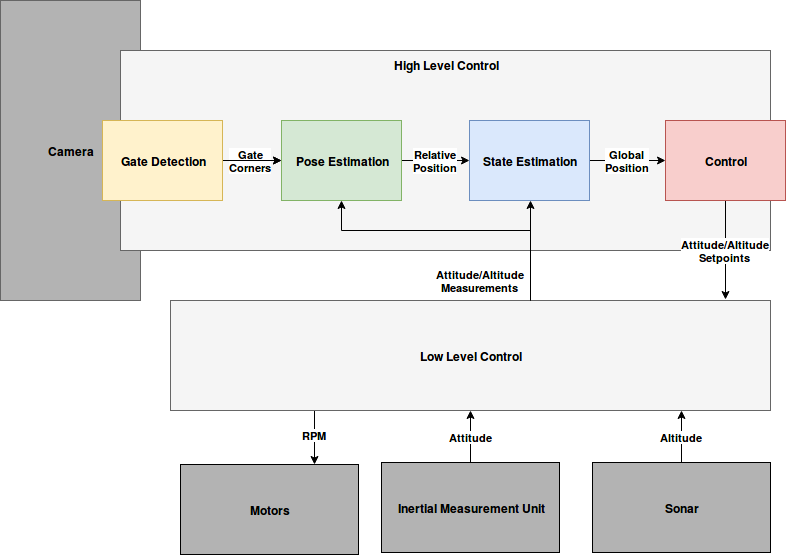
\includegraphics[width=0.8\textwidth]{fig/control_loop}
	\caption{Control Loop}
	\label{fig:control_loop}
\end{figure}

The high level control loop of this work is described in further detail. A first step detects the racing gate and yields the corner coordinates. These are used to estimate the relative position of the \ac{MAV} towards the gate. In the second step the visual measurements are fused with measurements of other sensors. In this case \ac{IMU} and a sonar deliver altitude and attitude data. This step yields a global position estimate of the \ac{MAV}. Combined with prior knowledge about the race court, the desired attitude and altitude required to fly the trajectory is calculated. The results are send as set points to the low level controller.

The hardware platform used to run the high level control loop is the \textit{JeVois} smart camera. It contains a 1.3 MP camera with 65 degree field of view. The processing units are a quad core ARM Cortex A7 processor with 1.35 GHz and a dual core MALI-400 GPU with 233 Mhz. In order to extent the field of view a 120 degree wide angle lens is mounted. In \Cref{fig:jevois} the camera is shown.

\begin{figure}[hbtp]
	\centering
	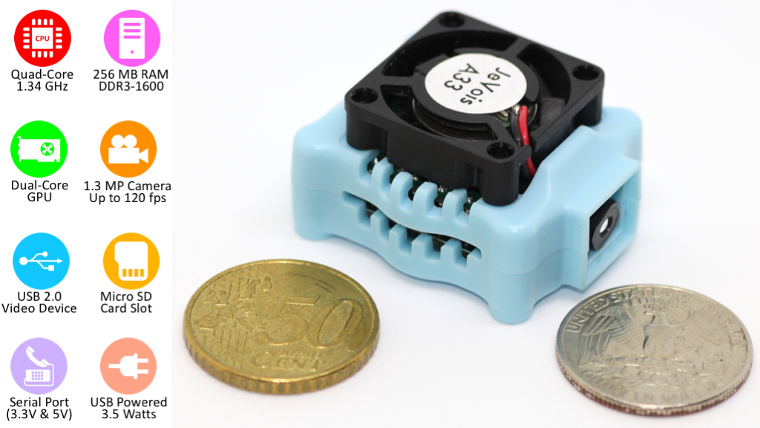
\includegraphics[width=0.5\textwidth]{fig/jevois}
	\caption{JeVois Camera}
	\label{fig:jevois}
\end{figure}



\if false
\section{Baseline}


\subsection{Experiment}

In order to compare the methods investigated in this thesis a baseline is determined. Therefore SnakeGate is evaluated on the datasets described in \Cref{sec:datasets}. In the experiment the color thresholds of the algorithm are fine tuned to the particular environment. The presented results are averages across 5 runs.


\subsection{Results}

The results in terms of precision and recall are summarized in \Cref{fig:snake_results_real}. It can be seen how the detector performs best in the Cyberzoo domain.

\begin{figure}
	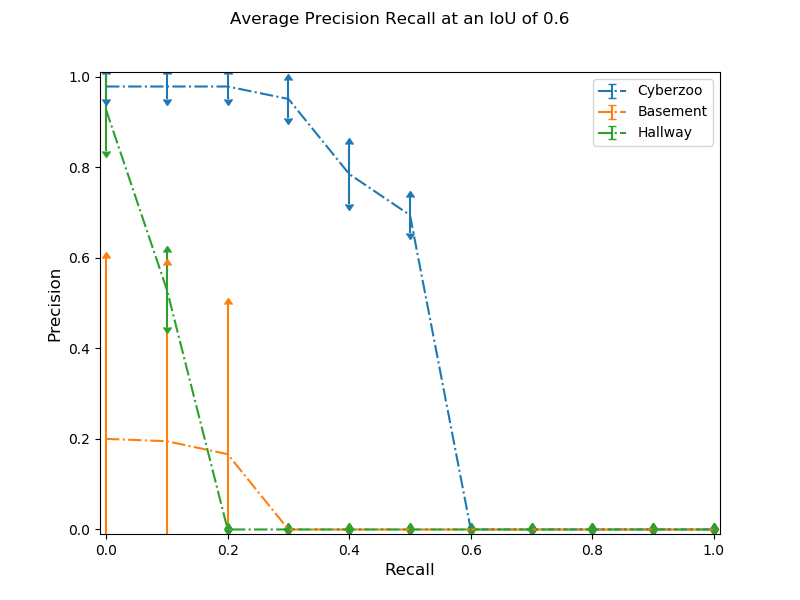
\includegraphics[width=0.8\textwidth]{fig/snake_results_real}
	\caption{Precision-Recall of Snake Gate on the datasets described in \Cref{sec:datasets}}
	\label{fig:snake_results_real}
\end{figure}

\fi